\documentclass[a4paper,12pt]{article}
%%\documentclass[a4paper,12pt]{revtex4}
\usepackage[hyphens]{url}
\usepackage{esvect}
\usepackage{amsmath}
\usepackage[]{units}

\usepackage{tabularx}
\usepackage{mathrsfs}
\usepackage{graphicx,color}
\usepackage{subfigure}
\usepackage{dcolumn}
\usepackage{bm}
\usepackage{slashed} % slash mark


\begin{document} \sloppy
\title{ZJpsi}
\author{}
\date{March 2015}
\maketitle

\begin{abstract}
We present a measurement of the probability of associated production of a Z boson and a $J\slash \psi$ meson given a Z boson at a center of mass energy of 8 \unit{TeV}. We  obtain the results with data corresponding to an integrated luminosity of about $19.8$ fb$^{-1}$.
\end{abstract}

\section{Introduction}
We measure the cross section of associated production of a Z boson and a $J\slash \psi$ meson. The predicted rate of this process in the Standard Model is quite small, but it is measurable with $19.8$ fb$^{-1}$ of integrated luminosity at $\sqrt{s} =$ \unit[8]{TeV}. Measurements of the $J\slash \psi$ are a good probe of quantum chromodynamics (QCD) and often are not initially well explained by theoretical predictions. For example, the initial cross section measured by the Tevatron was a factor of about 10 higher than the theory predicted. The leptonic decays of the Z and the $J\slash \psi$ provide a clean signal with hadron-hadron colliders.

\section{Theory}
Measuring $Prob(Z + J\slash \psi | Z)$ provides information on the production mechanism of the $J\slash \psi$. The evolution of a gluon into a $J\slash \psi$ is suppressed because a gluon is in a color octet state while a $J\slash \psi$ is in a color singlet state. There are two main models within Non-Relativistic QCD (NRQCD) that describe the production of a $J\slash \psi$. In the color singlet model (CSM), gluons can only evolve into quarkonia with the correct spin and quantum numbers. In contrast, in the color octet model (COM), the gluons can evolve into a state that at some later time radiates soft gluons to get the quantum numbers and spin state of a $J\slash \psi$. The COM is expected to have a much larger cross section than the CSM for this process. Theoretical papers written related to this topic include References 1-4.

From email communications with Song Mao: with the following experimental selection criteria on the final state particles the cross section for a Z and a $J\slash \psi$ was measured: 
\begin{center}
  \begin{tabular}{ | l | }
    \hline
    Requirement \\ \hline
    $J\slash \psi$ $p_T > 8.5$ \unit{GeV} \\ \hline
    $J\slash \psi$ $|y|<2.1$  \\ \hline
    Muon from $J\slash \psi$ $\mu |\eta| < 2.5$ \\ \hline
    $p_T$(first lepton from Z)$>25$ \unit{GeV} \\ \hline
    $p_T$(second lepton from Z)$> 15$ \unit{GeV}\\ \hline
    $|eta(lepton from Z)|<2.5$ \\ \hline
    $|m_(dilepton Z candidate)-90.2|< 10 $ \unit{GeV} \\ \hline
    \hline
  \end{tabular}
\end{center}
The cross section $*Br(J \slash \psi --> \mu\mu)$ differentially as a function of $J\slash \psi$ $p_T$ is:
\begin{center}
\begin{tabular}{cccccc}
                    &$^3S_1^{(8)}$ & $^3S_1^{(8)}$ & $^3S_1^{(1)}$  & $^3S_1^{(1)}$  \\
$p_T^{J/\psi}(GeV)$ &LO(fb)  &NLO(fb)&LO(fb)  &NLO(fb)        \\
\hline
    $8.5 \sim 10$   &0.0230  &0.0857 &0.0639  &0.0554    &    \\
    $10  \sim 14$   &0.0403  &0.1419 &0.0940  &0.0896    &    \\
    $14  \sim 18$   &0.0231  &0.0783 &0.0421  &0.0347    &    \\
    $18  \sim 30$   &0.0297  &0.0964 &0.0376  &0.0453    &    \\
    $30  \sim 100$  &0.0178  &0.0543 &0.0087  &0.0185    &    \\
\end{tabular}
\end{center}
The cross sections * $Br(J/\psi \to \mu^+\mu^-)*Br(Z \to \ell^+\ell^-)$ for the $pp \to J/\psi+Z$ process at the 8 \unit{TeV} LHC, where $Br(J/\psi \to \mu^+\mu^-) =5.93\% $ and $Br(Z \to \ell^+\ell^-) =6.729\% (\ell = e,\mu)$. The experimental selection criteria on the final state particles is applied. The input parameters are same as in Ref.arxiv.1102.0398. Add column 2 and column 4 together, the results is NLO cross section. Column 1 and column 3 together is the LO cross section results. NLO results are larger than LO.

From adding the NLO columns together (columns 2 and 4) and dividing by the cross section of the Z, the theoretical expectation is that the $Prob(Z + J\slash \psi | Z)$ is $0.854 \times 10^{-6}$.

\section{Analysis Procedure}
We reconstruct the Z boson when it decays to $e^+e^-$ or $\mu^+\mu^-$. We select the two highest $p_T$ muons (electrons) in the event with opposite charges. If the leptons pass the selection criteria and reconstruct a mass consistent with the Z mass, then we consider the event to contain a Z. We use the number of events with a Z passing all selection criteria and the number of events with both a Z and a $J\slash \psi$ passing all selection criteria to calculate $Prob(Z + J\slash \psi | Z)$, the probability that an event contains a Z and a $J\slash \psi$ given that the event contains a Z. This ratio cancels many of the systematic uncertainties, such as the systematic uncertainty on the efficiency of the Z and the uncertainty on the integrated luminosity.

We attempt to reconstruct the $J\slash \psi$ when it decays to $\mu^+\mu^-$. The analysis procedure to select $J\slash \psi$ dimuon candidates considers every pair of muons in the event (except if the two highest $p_{T}$ muons reconstruct to a mass consistent with that of a Z boson) to reconstruct potential $J\slash \psi$ dimuon candidates for the event. Then all $J\slash \psi$ dimuon candidates that pass the selection criteria are considered in the event. In practice, there is only one event with two $J\slash \psi$ dimuon candidates passing all selection criteria in addition to a Z in the event, while there are 138 events with at least one $J\slash \psi$ dimuon candidates in addition to a Z in the event. For the event with two $J\slash \psi$ dimuon candidates we consider both $J\slash \psi$ dimuon candidates in the analysis.

A large background for this analysis is events which contain a Z and a B-Hadron which decays to a $J\slash \psi$. When the $J\slash \psi$ arises from the decay of a B-hadron we term it a nonprompt $J\slash \psi$, in contrast to a prompt $J\slash \psi$ produced along with the Z. We can distinguish between prompt and nonprompt $J\slash \psi$ because of the long lifetime of the B-hadron (about $1.3$ ps). Another source of background is two muons from the dimuon mass continuum background which reconstruct a mass close to that of the $J\slash \psi$. These backgrounds are accounted for by a two-dimensional (2D) fit in $J\slash \psi$ candidate dimuon mass and lifetime.

\section{Selection Criteria}
We attempt to choose the selection criteria according to the official CMS guidelines when possible. We use the data sets: DoubleMuParked2012(ABCD){\_}22Jan2013-v1 and DoubleElectron2012(ABCD){\_}22Jan2013-v1. We determine which lumi sections to use with the golden lumi json file, \url{https://twiki.cern.ch/twiki/bin/viewauth/CMS/PdmV2012Analysis}. The leptons from the Z boson must have $p_{T} > 20$ \unit{GeV}. The probability that the two leptons come from the same vertex, vertex compatibility, must be $> 0.5\%$. Additionally, muons from the Z are required to pass the Tight Id requirement relative to the primary (highest $p_{T}$) vertex, as defined by \url{https://twiki.cern.ch/twiki/bin/view/CMSPublic/SWGuideMuonId}. The TightId requires that: the candidate is reconstructed as a global muon, its tracker track has transverse impact parameter $d_{xy} < 2$ mm with respect to the primary vertex, the longitudinal distance of the tracer track with respect to the primary vertex $d_{z} < 5$ mm, and a few other quality cuts to ensure that the particle is a muon.  Similarly, electrons from the Z are required to pass the Medium Id requirement, as defined by \url{https://twiki.cern.ch/twiki/bin/viewauth/CMS/EgammaCutBasedIdentification}. The Medium Id requirement requires various quality cuts on to ensure isolated electrons reconstructed cleanly, and that the $|d0| (vtx) < 0.02 cm$ and $|dZ| (vtx) < 0.1 cm$.  Electrons are subject to energy regression corrections as defined by \url{https://twiki.cern.ch/twiki/bin/viewauth/CMS/EgammaElectronEnergyScale#Electron_energy_scale_and_resolu}. The reconstructed Z mass must be between 60 and 120 \unit{GeV}.

In reconstructing the $J\slash \psi$, all oppositely charged muons are selected to form dimuon candidate $J\slash \psi$ particles, except if the two highest $p_{T}$ oppositely charged muons in the event reconstruct to have a mass in the Z mass window (60 to 120 \unit{GeV}), they are removed from the pool of muons which can form into a $J\slash \psi$ dimuon candidate. The $J\slash \psi$ is required to have mass between $2.85$ and $3.35$ \unit{GeV}, and also to have $|Rapidity_{J\slash \psi} |< 2.1$. The muons from a $J\slash \psi$ are required to pass SoftId relative to the primary vertex, as defined by \url{https://twiki.cern.ch/twiki/bin/view/CMSPublic/SWGuideMuonId}. The SoftId requires various quality cuts on the muon's track and loose transverse and longitudinal impact parameter cuts, $d_{xy} < 0.3 cm$ and $d_z < 20 cm$ with respect to the primary vertex. The muon $p_{T}$ of both muons is required to be $> 3.5$ \unit{GeV}. The muons' $| \eta | < 2.1$. The muons must have a vertex compatibility $> 0.5\%$. In addition, the $J\slash \psi$ is required to be within 1 \unit{cm} in the $z$-direction (along the beam-line) of the Z boson's reconstructed vertex.


\section{Fitting}
We distinguish between prompt and nonprompt $J\slash \psi$ by measuring the $J\slash \psi$ transverse lifetime. The lifetime in the transverse plane $t_{xy} = (m^{J\slash \psi} \slash p_{T}^{J\slash \psi}) \cdot L^{J\slash \psi}_{xy}$ where $L^{J\slash \psi}_{xy} = (\vv{r}_{T} \cdot \vv{p}_{T}^{J\slash \psi})\slash|\vv{p}_{T}^{J\slash \psi}|$, and $\vv{r}_{T}$ is the transverse distance between the reconstructed Z boson position and $J\slash \psi$ vertex position. Because the $p_T$ of the $J\slash \psi$ is used instead of the $p_T$ of the B-hadron, this transverse lifetime will not necessarily agree perfectly with the expected lifetime of the B-hadron.

We perform a 2D fit to distinguish Z + prompt $J\slash \psi$ from Z + nonprompt $J\slash \psi$ and/or Z + dimuon mass continuum background. The 2D fit is done in dimuon $t_{xy}$ and dimuon mass for an event with a Z and $J\slash \psi$ dimuon candidate passing all selection criteria. Because the expected cross section of $Z + J\slash \psi$ is very small, the fit is first performed on a large control sample of inclusive $J\slash \psi$. The control sample is collected with the dimuon8 trigger using the MuOniaParked-Run2012B-22Jan2013-v1 data set. This sample of inclusive $J\slash \psi$ determines the shapes of the templates used to fit the signal and background components of $Z + J\slash \psi$ dimuon candidate data.

The dimuon lifetime fit for signal is the sum of two Gaussian functions with a common mean but different standard deviations. The dimuon lifetime background, nonprompt $J\slash \psi$, component is modelled by an exponential decay smeared with a Gaussian resolution function. The dimuon mass signal is modelled by the sum of a Gaussian and a crystal ball with a common mean (to account for changing resolution with $J\slash \psi$ rapidity and for final state radiation (FSR)). The dimuon mass continuum background is modelled by an exponential decay. The relative fractions of: prompt $J\slash \psi$, nonprompt $J\slash \psi$, prompt continuum dimuon background, and nonprompt dimuon background are free to float with the requirement that these fractions sum to 1. The number of signal $J\slash \psi$ is then determined by multiplying the number of events in the 2D histogram by the fraction of prompt $J\slash \psi$.

The overall fit is:
\begin{multline}
 F(m,t) = f_{ms} \cdot f_{ts} \cdot MS(m) \ast TS(t) + f_{ms} \cdot f_{tb} \cdot MS(m) \ast TB(t) \\
 + f_{mb} \cdot f_{ts} \cdot MB(m) \ast TS(t) + f_{mb} \cdot f_{tb} \cdot MB(m) \ast TB(t)
\end{multline}
where $f_{(m,t)(s,b)}$ is the fraction of (mass,lifetime)(signal,background), $MS(m)$ is the mass signal template $MB(m)$ is the mass background template, $TS(t)$ is the lifetime signal template and $TB(T)$ is the lifetime background template. The templates ($MS(m)$, $MB(m)$, $TS(t)$ and $TB(T)$) are fixed from the fit to the inclusive $J\slash \psi$ sample, while ($f_{ts}$, $f_{ms}$, $f_{ts}$ and $f_{tb}$) are free to float when fitting the $Z+J\slash \psi$ data.

The fit is performed in 5 bins of $p_{T}$ because the $J\slash \psi$ lifetime resolution changes with $p_{T}$. Additionally, binning in $p_T$ mitigates the bias in the efficiency and acceptance calculated with inclusive $J\slash \psi$ MC because of the potentially different $p_T$ distributions between inclusive $J\slash \psi$ and $J\slash \psi$ in events which also contain a Z. Once the fit is performed, the parameters other then the relative fractions are fixed, and then applied to determine the number of signal $J\slash \psi$ in events which also contain a Z boson. For the inclusive sample, the fit parameters are (integrated over all $p_{T}$):
\begin{center}
  \begin{tabular}{ | l | l | l | }
    \hline
    Floating Parameter        &  Value      & Error    \\ \hline
    mass mean                 &  3.0928e+00 & 1.09e-05 \\ \hline
    mass cball alpha          &  1.3233e+00 & 2.35e-03 \\ \hline
    mass cball n              &  8.0000e+01 & 6.28e-01 \\ \hline
    mass cball sigma          &  3.8280e-02 & 5.37e-05 \\ \hline
    mass gauss sigma          &  2.0588e-02 & 4.21e-05 \\ \hline
    mass cball frac           &  5.9152e-01 & 2.18e-03 \\ \hline
    mass bg slope             &  -2.1970    & 7.72e-03 \\ \hline
    t gauss mean              &  2.8003e-03 & 4.39e-05 \\ \hline
    t gauss1 sigma            &  6.3727e-02 & 1.15e-04 \\ \hline
    t gauss2 sigma            &  1.2694e-01 & 4.00e-04 \\ \hline
    t frac gauss1             &  6.5160e-01 & 2.75e-03 \\ \hline
    t bg decay lifetime       &  9.8571e-01 & 6.46e-04 \\ \hline
    t bg smear gauss sigma    &  1.3776e-01 & 6.53e-04 \\ \hline
    m sig t sig frac          &  5.9533e-01 & 2.05e-04 \\ \hline
    m sig t bg recursive frac &  7.5989e-01 & 3.51e-04 \\ \hline
    m bg t sig recursive frac &  2.8428e-01 & 8.54e-04 \\ \hline
    \hline
  \end{tabular}
\end{center}

We use these fit parameters to fit the data when there is a Z boson and a $J\slash \psi$ in the event. The fit results (integrated over the entire $p_{T}$ range) are shown in the table below.
\begin{center}
  \begin{tabular}{ | l | l | l | }
      \hline
      Floating Parameter                                 &  Value      & Error    \\ \hline
      m sig t sig frac (Z$\rightarrow\mu\mu$)            &  2.0928e-01 & 6.61e-02 \\ \hline
      m sig t bg recursive frac (Z$\rightarrow\mu\mu$)   &  6.1533e-01 & 7.47e-02 \\ \hline
      m bg t sig recursive frac (Z$\rightarrow\mu\mu$)   &  5.8302e-01 & 1.38e-01 \\ \hline
      m sig t sig frac (Z$\rightarrow$ee)                &  1.6258e-01 & 8.36e-02 \\ \hline
      m sig t bg recursive frac (Z$\rightarrow$ee)       &  6.6390e-01 & 1.01e-01 \\ \hline
      m bg t sig recursive frac (Z$\rightarrow$ee)       &  6.0569e-01 & 1.98e-01 \\ \hline
      \hline
  \end{tabular}
\end{center}

The number of events from the mass signal and t signal is computed from the fit fraction and the number of events in the histogram. The number of events, accounting for fit uncertainty and statistical uncertainty and summing over the 5 $p_T$ bins, for Z $\rightarrow\mu\mu + J\slash \psi \rightarrow\mu\mu $ is $19.64 \pm 5.94$. For Z $\rightarrow ee + J\slash \psi \rightarrow\mu\mu$ the number of events is $8.29 \pm 3.80 $. After correcting for acceptance $\ast$ efficiency, as described in the section on acceptance, the corrected number of events for Z $\rightarrow\mu\mu + J\slash \psi \rightarrow\mu\mu $ is $49.51 \pm 14.19$. For Z $\rightarrow ee + J\slash \psi \rightarrow\mu\mu$ the corrected number of events is $15.09 \pm 7.16$. This compares to $8.481 \times 10^{6}$ $Z \rightarrow\mu\mu$ events in the data set or $5.274 \times 10^{6}$  $Z\rightarrow ee$ events in the data set, which can be used to compute $Prob(Z + J\slash \psi | Z)$. The $Prob(Z\rightarrow\mu\mu + J\slash \psi\rightarrow\mu\mu | Z\rightarrow\mu\mu)$ is $5.84 \pm 1.67 \times 10^{-6}$. The $Prob(Z\rightarrow ee + J\slash \psi\rightarrow\mu\mu | Z\rightarrow ee)$ is $2.86 \pm 1.36 \times 10^{-6}$.

The results of signal for each $p_T$ bin are shown in the table below.
\begin{center}
  \begin{tabular}{ | l | p{2cm} | p{2cm} | p{2cm} | p{2cm} | l | }
    \hline
    $p_T$ \unit{GeV} & Z$\rightarrow\mu\mu$ + $J\slash\psi\rightarrow\mu\mu$ Events & Z$\rightarrow\mu\mu$ + $J\slash\psi\rightarrow\mu\mu$ Error & Z$\rightarrow$ee +  $J\slash\psi\rightarrow\mu\mu$ Events & Z$\rightarrow$ee + $J\slash \psi\rightarrow\mu\mu$ Error & Eff$*$Acc \\ \hline
    8.5-10 & 7.86 & 3.16 & 0     & 0.80   & 0.199279 \\ \hline
    10-14  & 7.65 & 3.34 & 4.27  & 2.35   & 0.321599 \\ \hline
    14-18  & 0    & 1.31 & 0.43  & 1.07   & 0.470349 \\ \hline
    18-30  & 0    & 1.58 & 3.60  & 2.61   & 0.576247 \\ \hline
    30-100 & 4.13 & 3.14 & 0     & 0.53   & 0.705206 \\ \hline
    \hline
  \end{tabular}
\end{center}

\section{Acceptance}
We calculate the acceptance and efficiency to reconstruct a $J\slash\psi$ by generating prompt $J\slash \psi$ MC. Although there may be some bias when comparing events with a Z and a $J\slash \psi$ to events where $J\slash \psi$ are generated without a Z, binning the analysis in bins of $p_T$ and using a relatively high threshold for $J\slash \psi$ $p_T$ should somewhat help alleviate this. In addition, it is non-trivial to generate accurate Z+$J\slash \psi$ MC. Because the final measurement is of $Prob(Z + J\slash \psi | Z)$, the acceptance and efficiency of the Z boson will not play a large role in the measurement we make. We correct for possible differences between data and MC by using scale factors to weight the MC generated and reco $p_T$ and $\eta$ distributions to more accurately reflect the distributions in data (we weight the numerator and denominator by a scale factor measured with tag-and-probe using muons from a $J\slash \psi$ by CMS-DP-2014-020).

The acceptance $\ast$ efficiency is determined by the ratio of the number of reconstructed $J\slash \psi$ that pass all selection criteria, except the requirement that the $J\slash \psi$ vertex position is within $1$ \unit{cm} in the $z$-direction of the reconstructed Z boson vertex, and the number of generated $J\slash \psi$. The acceptance and efficiency are calculated for 5 bins of $J\slash \psi$ $p_T$ and with the requirement that the $J\slash \psi$ rapidity is within the selection criteria. From observing the difference between reconstructed $J\slash \psi$ dimuon vertex position and generated truth $J\slash \psi$ dimuon vertex position we believe that the requirement that the $J\slash \psi$ vertex is within $1$ \unit{cm} in the $z$-direction of the Z vertex keeps virtually all of the signal. This acc $\ast$ eff is calculated in bins of $p_T$ in order to account for potential differences in the distribution of $p_T$ between the $J\slash \psi$ from an inclusive $J\slash \psi$ sample and from events that contain a Z and a $J\slash \psi$.

One significant source of uncertainty in determining the acceptance of the $J\slash \psi$ is its polarization. The polarization of the $J\slash \psi$ affects the $p_T$ and $\eta$ balance of the muons from the $J\slash \psi$, polarizations with more balanced muons have a higher acceptance. The MC is generated with the assumption that the $J\slash \psi$ is unpolarized, deviations from this assumption are taken as a systematic uncertainty. The effect of polarization is determined by reweighting the MC events according to:
\begin{equation} \label{eq2}
  \frac{\mathrm d N}{\mathrm d \cos{\theta^{\star}}} \propto 1 + \lambda_{\theta} \cos^2{\theta^{\star}}
\end{equation}
where $\theta^{\star}$ is the angle between the direction of the positive muon momentum in the $J\slash \psi$ decay frame and the $J\slash \psi$ line of flight. The value of $\lambda_{\theta}$, which is $0$ in the unpolarized scenario, can range from -1 to 1. This causes a difference in acceptance of about 30 percent. This only considers the leading order effect of polarization, and only in the $\theta^{\star}$ direction.

\begin{center}
  \begin{tabular}{ | l | l | l | l | }
    \hline
    $p_T$ \unit{GeV} & Unpolarized $(\lambda = 0)$ & Long $(\lambda = -1)$ & Transverse $T_{+0}$ $(\lambda = 1)$ \\ \hline
    8.5-10 & 0.199279 & 0.28599   & 0.155924  \\ \hline
    10-14  & 0.321599 & 0.450387  & 0.257241  \\ \hline
    14-18  & 0.470349 & 0.628361  & 0.391154  \\ \hline
    18-30  & 0.576247 & 0.731672  & 0.498353  \\ \hline
    30-100 & 0.705206 & 0.81846   & 0.647919  \\ \hline
    \hline
  \end{tabular}
\end{center}

\section{Backgrounds}
The main backgrounds for our signal include: Z + nonprompt $J\slash \psi$, Z + dimuon continuum background, pileup and Double Parton Scattering (DPS). The first two backgrounds listed are accounted for through the 2D fit described in the section on fitting. Pileup, in which the Z and the $J\slash \psi$ come from different vertexes in the same event, is estimated by repeating the analysis with the pileup cut inverted. We invert the cut requiring the $J\slash \psi$ and the Z to be within 1 \unit{cm} in the $z$-direction, to select a sample dominated by pileup. From this sample we estimate the number of pileup events in the signal region by extrapolating from the background region. We estimate the background from DPS from the cross section of the $J\slash \psi$ and the effective cross section for DPS for p-p collisions.

Pileup is determined to have $16.98 \pm 9.30$ in the $Z\rightarrow\mu\mu$ channel for the inverted cut, and after correcting for acceptance$\ast$efficiency there are $43.80 \pm 17.24$ events. In the $Z\rightarrow ee$ channel there are $7.77 \pm 4.56$ events, after acceptance $\ast$ efficiency correction, there are $20.00 \pm 9.84$ events. From a Gaussian fit of vertex position in the inclusive $J\slash \psi$ data set, the fraction of pileup vertexes that are excluded by the vertex position in the $z$-direction is $88.4\%$. Because the pileup in the signal region is related to the pileup events in the background region by $N_{sig} = N_{bg} \cdot \frac{frac(sig)}{frac(bg)}$, the $Prob(Z\rightarrow\mu\mu + J\slash \psi\rightarrow\mu\mu | Z\rightarrow\mu\mu)$ is $0.68 \pm 0.27 \times 10^{-6}$. The pileup $Prob(Z\rightarrow ee + J\slash \psi\rightarrow\mu\mu | Z\rightarrow ee)$ is $0.50 \pm 0.25 \times 10^{-6}$.

The $Prob(Z + J\slash \psi | Z)$ because of DPS is calculated by:
\begin{equation}
Prob(Z+J\slash\psi | Z) = \frac{\sigma_{J\slash\psi}}{\sigma_{eff}}
\end{equation}
where $\sigma_{J\slash\psi}$ is the $J\slash \psi$ cross section and $\sigma_{eff}$ is the effective cross section for DPS, which does not depend on the specific processes observed. We estimate the prompt $\sigma_{J\slash\psi}$ for our selection criteria from $[arXiv:1104.3038v2]$ to be $24.44 \pm 1.44$ (stat) $\pm 2.86$ (syst) $\pm 6.42$ (polarization uncertainty) \unit{nb}. This measurement was made at 7 \unit{TeV}, so we extrapolate it to 8 \unit{TeV}. From [arXiv:1103.2394v3] $f(\sqrt{s}) = A \cdot (\sqrt{s\slash s_{0}})^b$ where $A = 124 \pm 9 $ \unit{nb}, $b = 0.60 \pm 0.06$ and $\sqrt{s_0} = 1$ \unit{TeV}. From [arXiv:1312.5729v2] $\sigma_{eff} = 20.7 \pm 0.8$ (stat.) $\pm 6.6$ (syst.) \unit{mb}. Therefore the $Prob(Z + J\slash \psi | Z)$ because of DPS is $1.28 \pm 0.56 \times 10^{-6}$.

\section{Summary}
If we subtract the backgrounds of pileup and DPS, the measured $Prob(Z\rightarrow\mu\mu + J\slash \psi\rightarrow\mu\mu | Z\rightarrow\mu\mu)$ is $3.88 \pm 1.78 \times 10^{-6}$. The measured $Prob(Z\rightarrow ee + J\slash \psi\rightarrow\mu\mu | Z\rightarrow ee)$ with background subtracted is $1.08 \pm 1.49 \times 10^{-6}$. The expected theoretical probability from communications with Song Mao, is $0.854 \times 10^{-6}$. 

\section{Cross Checks}
I have made several plots to cross check and examine the data. 

\begin{figure}[]
    \centering
      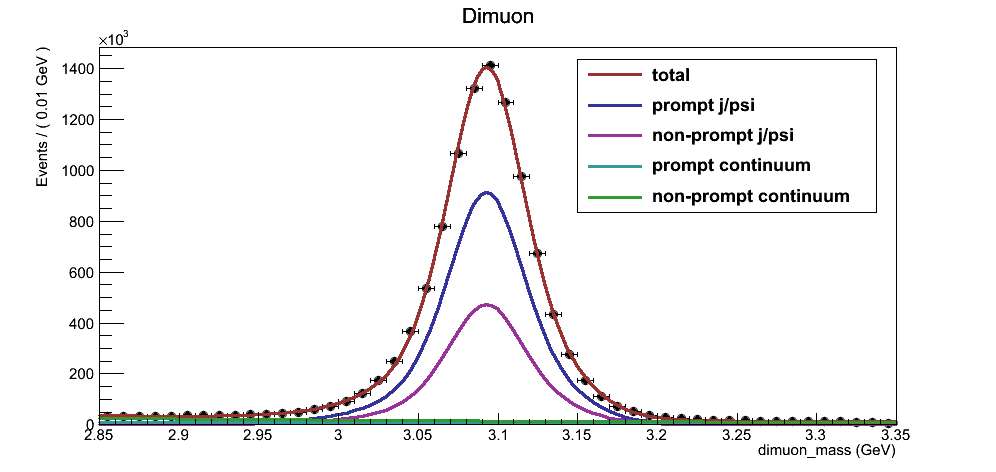
\includegraphics[scale=0.4]{Images/inclusive_jpsi_mass0.png}
  \caption{$J\slash\psi$ inclusive $J\slash\psi$ mass}
\end{figure}
\begin{figure}[]
    \centering
      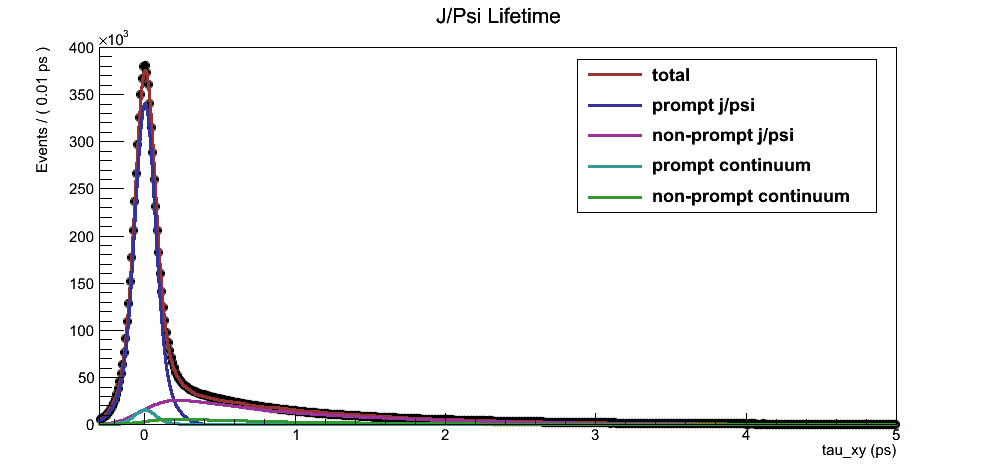
\includegraphics[scale=0.4]{Images/inclusive_jpsi_tau_xy0.png}
      %%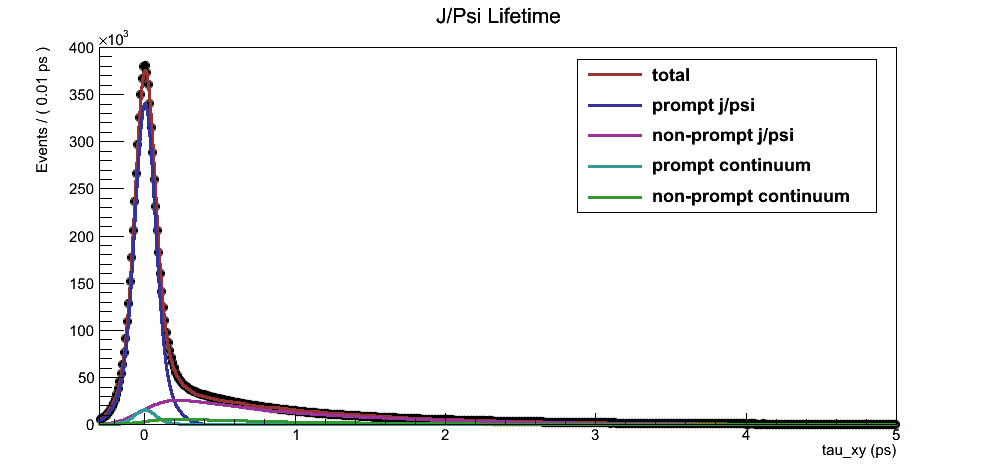
\includegraphics[width=0.5\textwidth]{Images/inclusive_jpsi_tau_xy0.png}
    \caption{$J\slash\psi$ inclusive lifetime}
\end{figure}

\begin{figure}[]
    \centering
      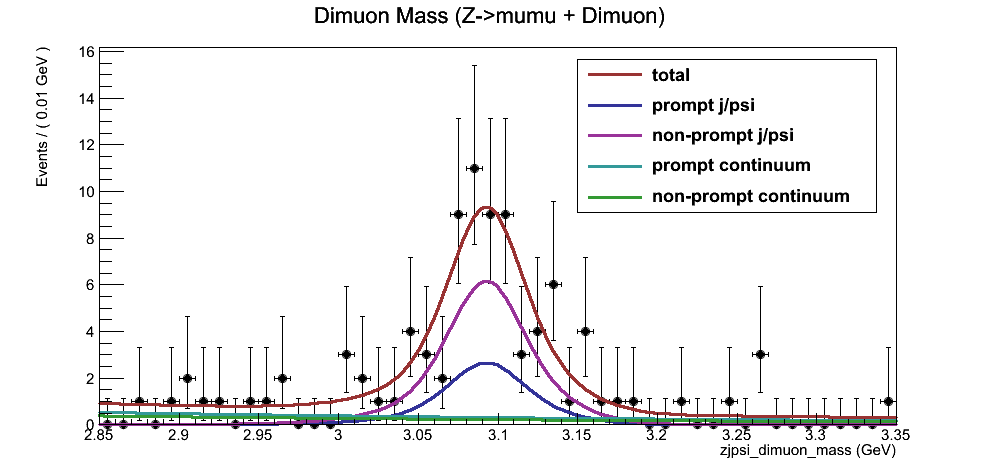
\includegraphics[scale=0.4]{Images/ztomumu_jpsi_dimuon_mass0.png}
    \caption{Z to $\mu\mu$ and $J\slash\psi$ mass}
\end{figure}
\begin{figure}[]
    \centering
      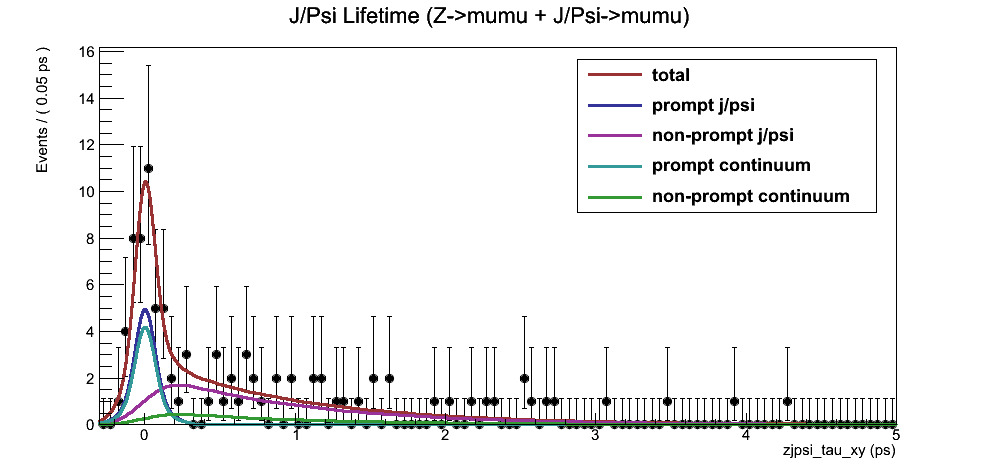
\includegraphics[scale=0.4]{Images/ztomumu_jpsi_tau_xy0.png}
    \caption{Z to $\mu\mu$ and $J\slash\psi$ lifetime}
\end{figure}

\begin{figure}[]
    \centering
      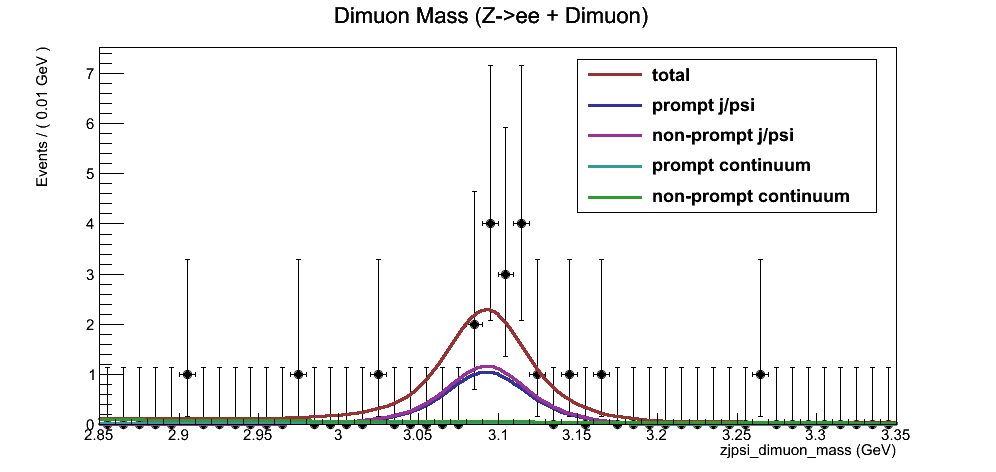
\includegraphics[scale=0.4]{Images/ztoee_jpsi_dimuon_mass0.png}
    \caption{Z to ee and $J\slash\psi$ mass}
\end{figure}
\begin{figure}[]
    \centering
      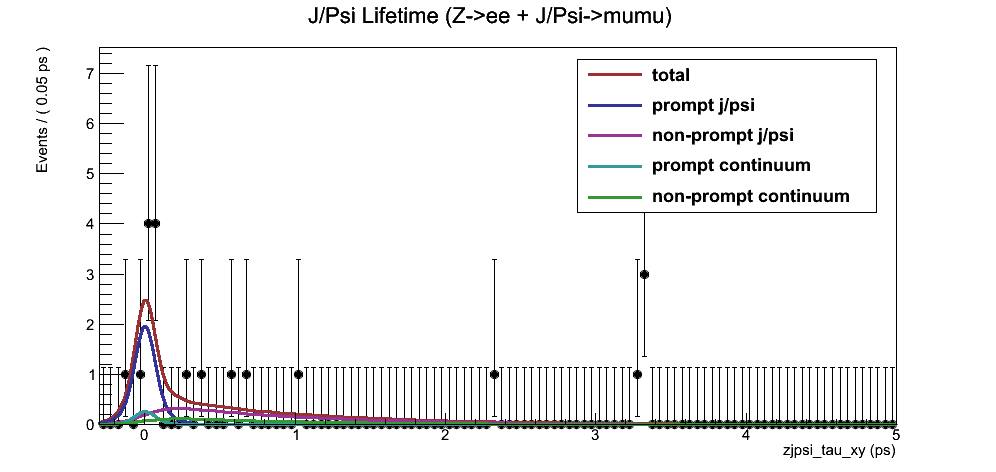
\includegraphics[scale=0.4]{Images/ztoee_jpsi_tau_xy0.png}
    \caption{Z to ee and $J\slash\psi$ lifetime}
\end{figure}


%%MC plots - probably too many of these!
\begin{figure}[]
    \centering
      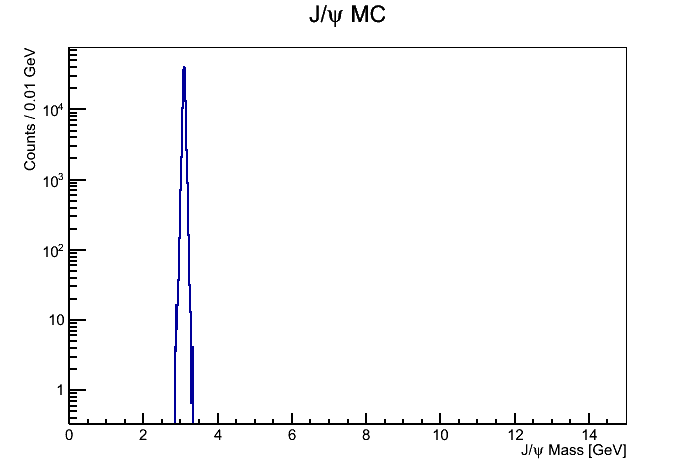
\includegraphics[scale=0.5]{Images/jpsi_mass.png}
    \caption{}
\end{figure}
\begin{figure}[]
    \centering
      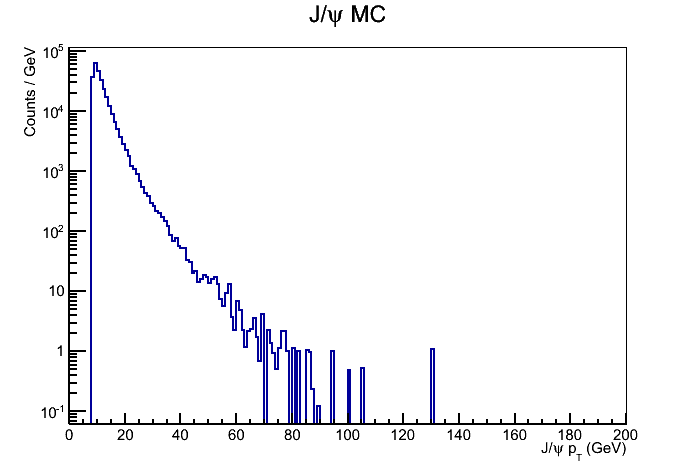
\includegraphics[scale=0.5]{Images/jpsi_pt.png}
    \caption{}
\end{figure}
\begin{figure}[]
    \centering
      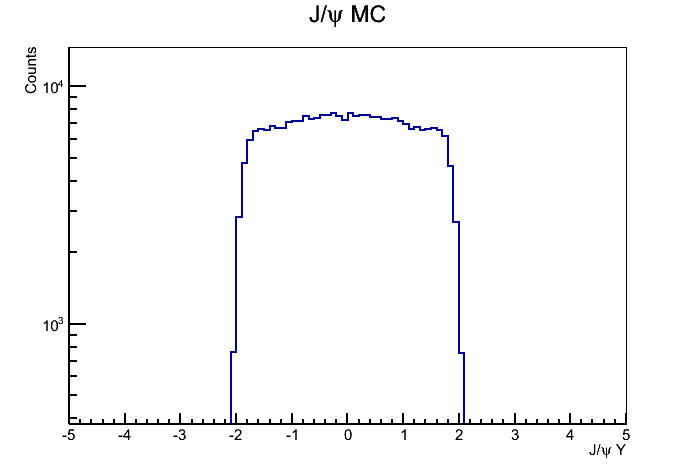
\includegraphics[scale=0.5]{Images/jpsi_rap.png}
    \caption{}
\end{figure}
\begin{figure}[]
    \centering
      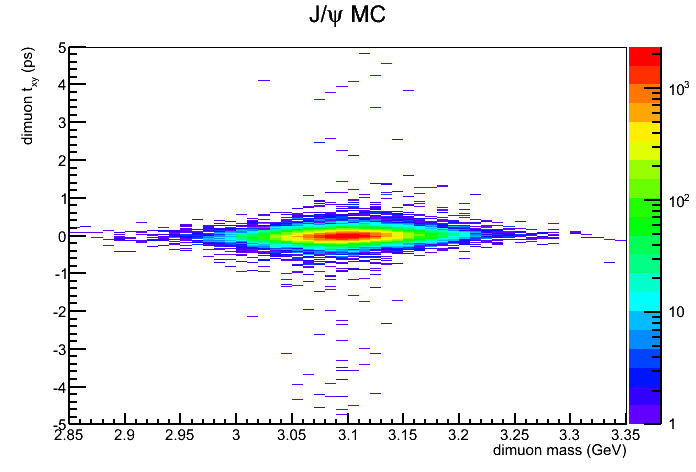
\includegraphics[scale=0.5]{Images/dimuon_mass_vs_dimuon_tau_xy.png}
    \caption{}
\end{figure}
\begin{figure}[]
    \centering
      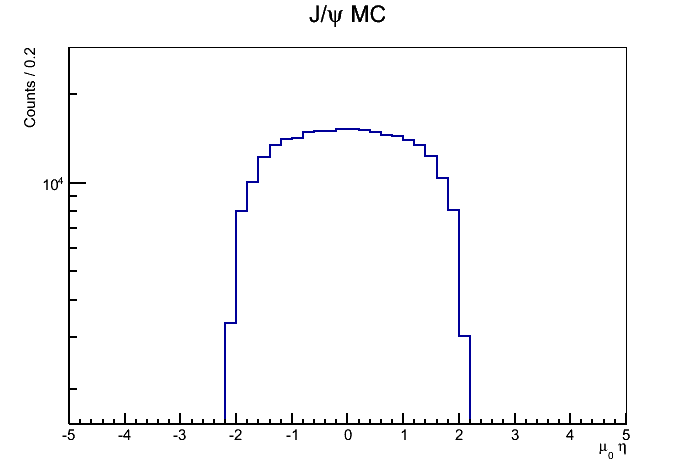
\includegraphics[scale=0.5]{Images/mu0_eta.png}
    \caption{}
\end{figure}
\begin{figure}[]
    \centering
      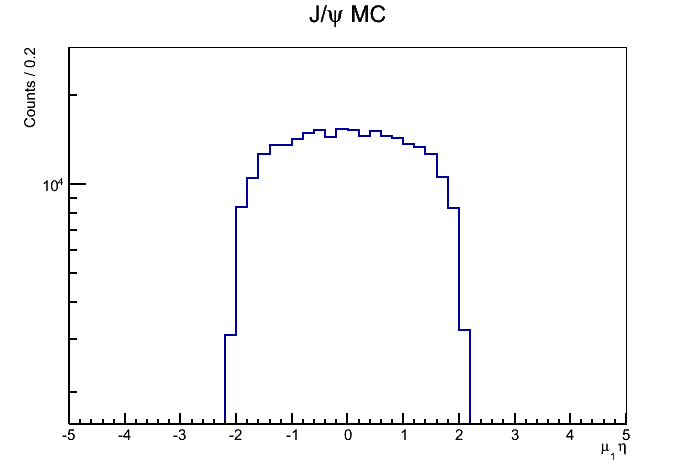
\includegraphics[scale=0.5]{Images/mu1_eta.png}
    \caption{}
\end{figure}
\begin{figure}[]
    \centering
      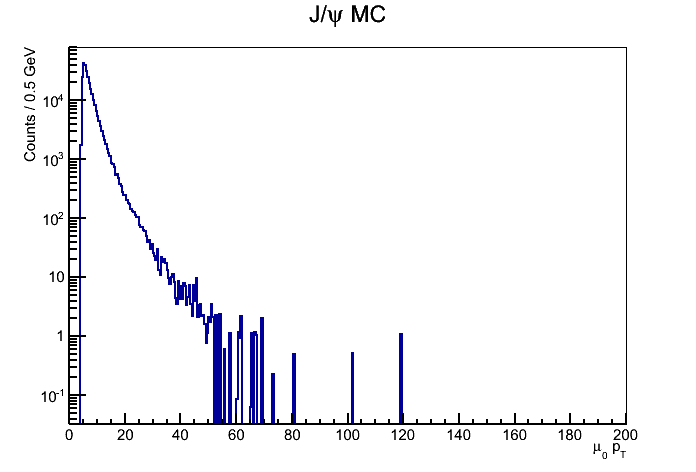
\includegraphics[scale=0.5]{Images/mu0_pT.png}
    \caption{}
\end{figure}
\begin{figure}[]
    \centering
      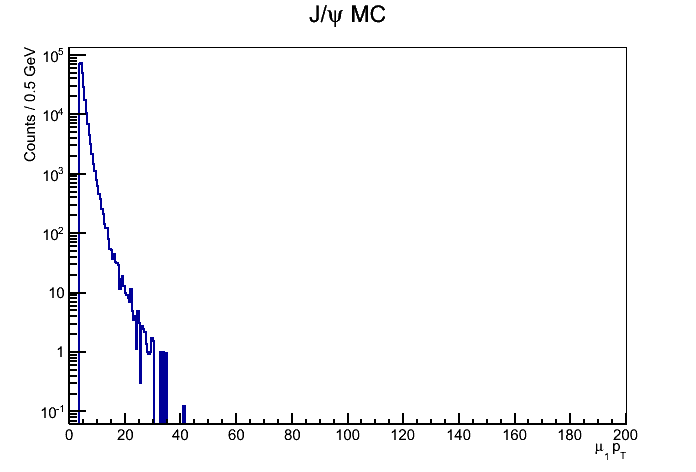
\includegraphics[scale=0.5]{Images/mu1_pT.png}
    \caption{}
\end{figure}
\begin{figure}[]
    \centering
      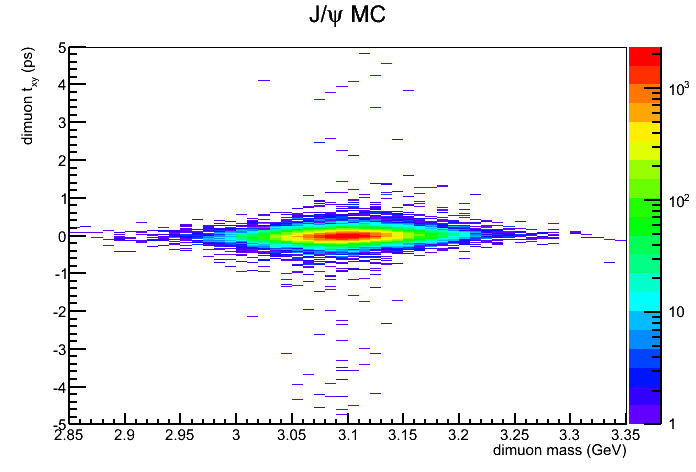
\includegraphics[scale=0.5]{Images/dimuon_mass_vs_dimuon_tau_xy.png}
    \caption{}
\end{figure}
\begin{figure}[]
    \centering
      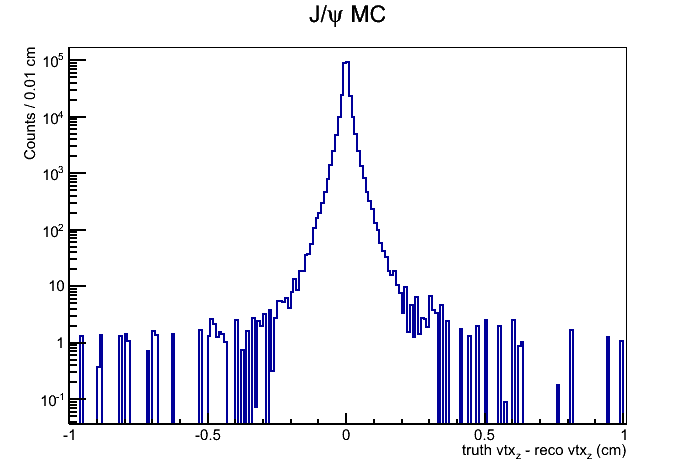
\includegraphics[scale=0.5]{Images/jpsi_truth_vtx_z_minus_jpsi_reco_vtx_z.png}
    \caption{}
\end{figure}
\begin{figure}[]
    \centering
      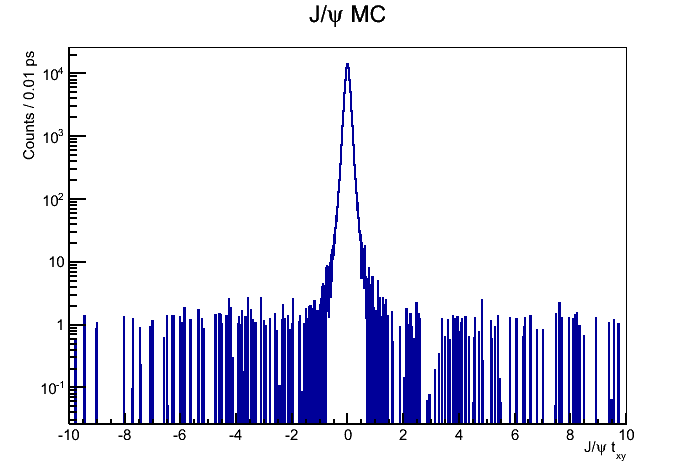
\includegraphics[scale=0.5]{Images/jpsi_tau_xy_very_fine_al.png}
    \caption{}
\end{figure}
\begin{figure}[]
    \centering
      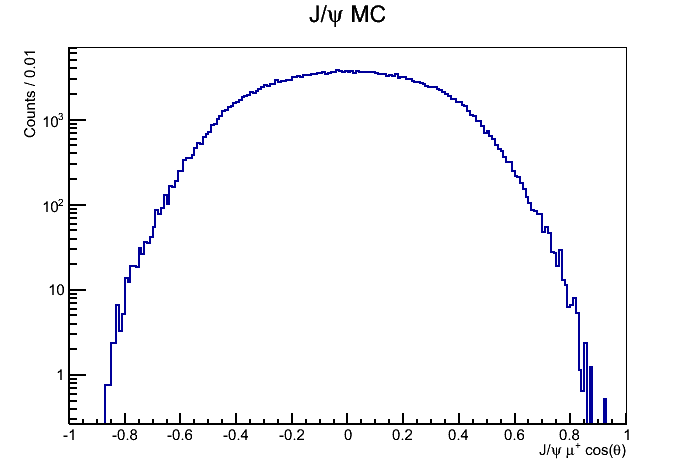
\includegraphics[scale=0.5]{Images/jpsi_cos_mu_plus.png}
    \caption{}
\end{figure}

%%Data Plots



%%
%%% useful plots:
%%mass, pT, eta distributions of Z and J/Psi
%%Fit plots
%%MC acceptance and efficiency plots
%%Other miscellaneous plots%
%%

References:
Ref1: $http://arxiv.org/abs/1309.4736v3$ (T. Alexopoulos, S. Leontsinis)
Ref2: $[arXiv:1102.0398v3]$ (Song Mao et al)
Ref3: $[arXiv:hep-ph/0208104v1]$ (Caesar P. Palisoc, Lennart Zwirner)
Ref4: $[arXiv:1210.2430v1]$ (Bin Gong et al)

\end{document}
